\chapter{Exploratory Data Analysis}\label{ch:eda}

This chapter answers the descriptive question, \emph{what happened?}, and begins to answer \emph{why}. All
results were computed on the full cleaned dataset by \texttt{eda.py}.

\section{Overall performance and growth}
Over the whole period, the company sold \TotalUnits million units in \NRows orders, worth \BDT\TotalSales
million in net sales. The average order was worth \BDT\AOV, and discounts averaged \AvgDiscount\% of gross
value, a cost of \BDT\DiscountCost million. \Cref{tab:annual} and \cref{fig:trend} show steady growth. Between
the first and the last complete year (2020--2025), net sales grew at a compound annual rate of \CAGRSales\%.
Sales in January--September 2026 were \YTDGrowth\% above the same months of 2025.

\begin{table}[htbp]
\centering
\small
\caption{Annual performance summary, 2020--2026}
\label{tab:annual}
\begin{adjustbox}{max width=\linewidth}
\begin{tabular}{lrrrrrrr}
\toprule
\textbf{Year} & \textbf{Orders} & \textbf{Units} & \textbf{Net sales (BDT M)} & \textbf{AOV (BDT)} & \textbf{Avg price} & \textbf{Disc. \%} & \textbf{YoY \%} \\
\midrule
2020 & 74,788 & 398,005 & 28.62 & 382.7 & 72.0 & 2.34 & -- \\
2021 & 73,636 & 418,104 & 37.02 & 502.7 & 88.6 & 2.35 & +29.3 \\
2022 & 73,898 & 440,150 & 41.00 & 554.8 & 93.4 & 2.34 & +10.8 \\
2023 & 73,598 & 460,465 & 46.17 & 627.3 & 100.5 & 2.36 & +12.6 \\
2024 & 74,282 & 486,293 & 53.03 & 713.9 & 109.8 & 2.35 & +14.9 \\
2025 & 74,442 & 507,262 & 61.78 & 829.9 & 122.3 & 2.35 & +16.5 \\
2026* & 55,356 & 381,678 & 50.75 & 916.8 & 133.8 & 2.34 & -- \\
\bottomrule
\end{tabular}
\end{adjustbox}
\par\smallskip\parbox{0.92\linewidth}{\footnotesize\emph{Note:} * 2026 covers January--September only, so growth is not computed for it. AOV = average order value; price = mean unit selling price.}
\end{table}

\begin{figure}[htbp]\centering
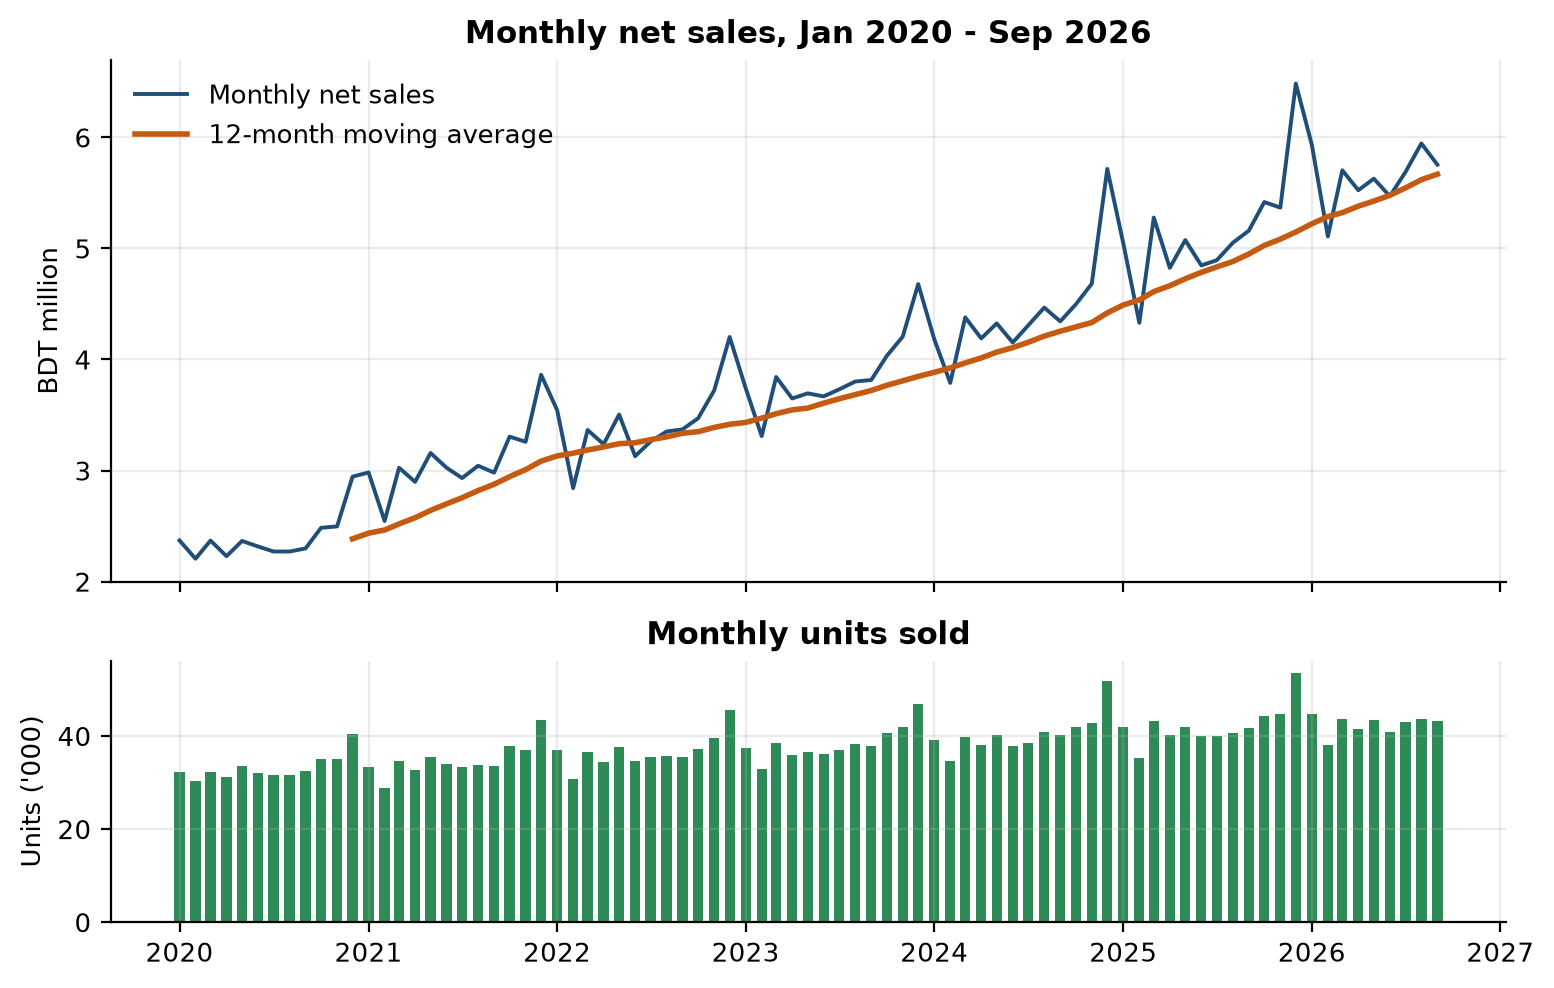
\includegraphics[width=\linewidth]{eda_monthly_trend}
\caption{Monthly net sales with 12-month moving average (top) and monthly units sold (bottom)}\label{fig:trend}
\end{figure}

\subsection{Where does growth come from?}
Units grew by only \CAGRUnits\% a year, whereas the average selling price grew by \CAGRPrice\% a year. Sales
growth can be decomposed exactly as $(1+g_{\text{sales}}) = (1+g_{\text{volume}})(1+g_{\text{price}})$.
\Cref{tab:pricevolume} and \cref{fig:pricevolume} show that, on average, about \AvgVolGrowth percentage points
of annual growth came from volume and \AvgPriceGrowth from price and product mix. The exceptional rise in 2021
coincides with the launch of higher-priced gift boxes, a mix effect. Later years reflect regular list-price
increases. This distinction matters for management: price-led growth cannot continue indefinitely without
eventually testing consumers' willingness to pay.

\begin{table}[htbp]
\centering
\small
\caption{Decomposition of annual sales growth into volume and price effects}
\label{tab:pricevolume}
\begin{adjustbox}{max width=\linewidth}
\begin{tabular}{lrrr}
\toprule
\textbf{Year} & \textbf{Sales growth \%} & \textbf{Volume growth \%} & \textbf{Avg price growth \%} \\
\midrule
2021 & +29.3 & +5.0 & +23.1 \\
2022 & +10.8 & +5.3 & +5.2 \\
2023 & +12.6 & +4.6 & +7.6 \\
2024 & +14.9 & +5.6 & +8.8 \\
2025 & +16.5 & +4.3 & +11.7 \\
\bottomrule
\end{tabular}
\end{adjustbox}
\par\smallskip\parbox{0.92\linewidth}{\footnotesize\emph{Note:} $(1+g_{sales}) = (1+g_{volume})(1+g_{price})$; price is net revenue per unit and therefore also reflects changes in product mix.}
\end{table}

\begin{figure}[htbp]\centering
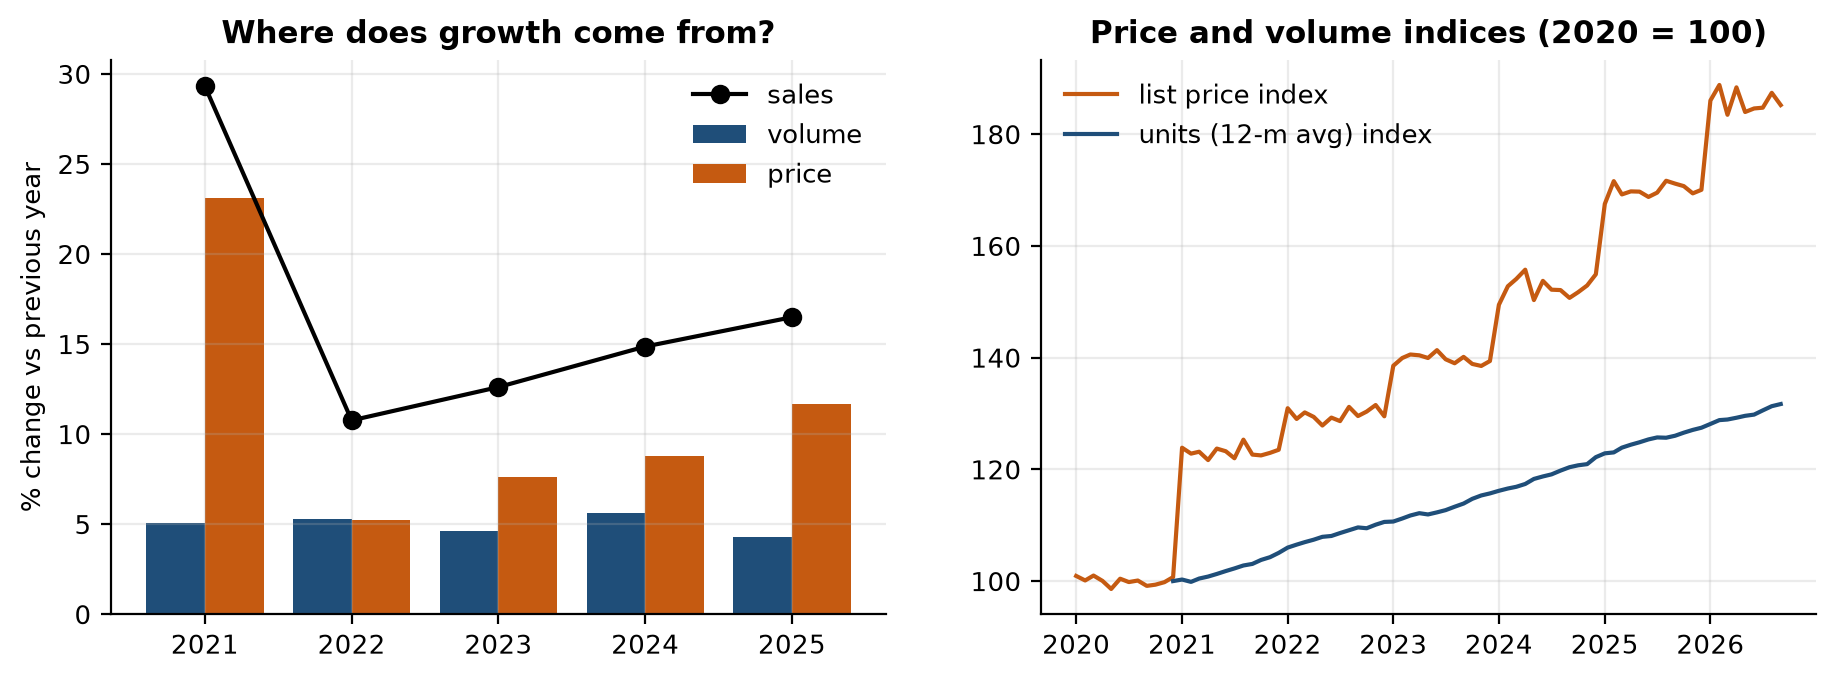
\includegraphics[width=\linewidth]{eda_price_volume}
\caption{Decomposition of growth (left) and price versus volume indices (right)}\label{fig:pricevolume}
\end{figure}

\subsection{Is demand sensitive to price?}
To separate the effect of price from that of general growth, the price elasticity of demand was estimated
with a fixed-effects regression on the product-month panel:
\[
  \log(\text{units}_{pt}) = \beta \log(\text{price}_{pt}) + \alpha_p + \gamma_{\text{year}(t)} + \delta_{\text{month}(t)} + \varepsilon_{pt}.
\]
The product effects $\alpha_p$ absorb differences in size between products. The year effects absorb common
market growth, and the month effects absorb seasonality. The estimated elasticity is
$\hat\beta = \Elasticity$, with a 95\% confidence interval from \ElasticityLo to \ElasticityHi (robust standard
errors; $p = \ElasticityP$; $R^2 = \ElasticityRtwo$). It is not significantly different from zero. Over the
observed range, demand therefore appears \emph{price-inelastic}. A naive regression without year effects gives
a misleading \emph{positive} elasticity of \ElasticityNaive, because prices and volumes both rose over time.
This is a textbook illustration of confounding, and the reason explanatory models need careful
specification \citep{shmueli2010}.

\section{Seasonality and calendar effects}
Sales show a clear annual cycle (\cref{fig:seasonality}). \PeakMonth is the strongest month, with a seasonal
index of \PeakIndex (average month = 100). October (\OctIndex) and November (\NovIndex) are also above average,
consistent with the year-end festive and gifting season. \TroughMonth is the weakest month (\TroughIndex). Part
of February's weakness is simply its shorter length: per trading day its index is \FebPerDay, while December's
per-day index remains high at \DecPerDay. A Kruskal--Wallis test on detrended daily sales confirms that
calendar month matters ($H = \KWMonthH$, $p<0.001$). By contrast, the day of the week has almost no effect: the
coefficient of variation of average daily sales across weekdays is only \DowCV\%.

\begin{figure}[htbp]\centering
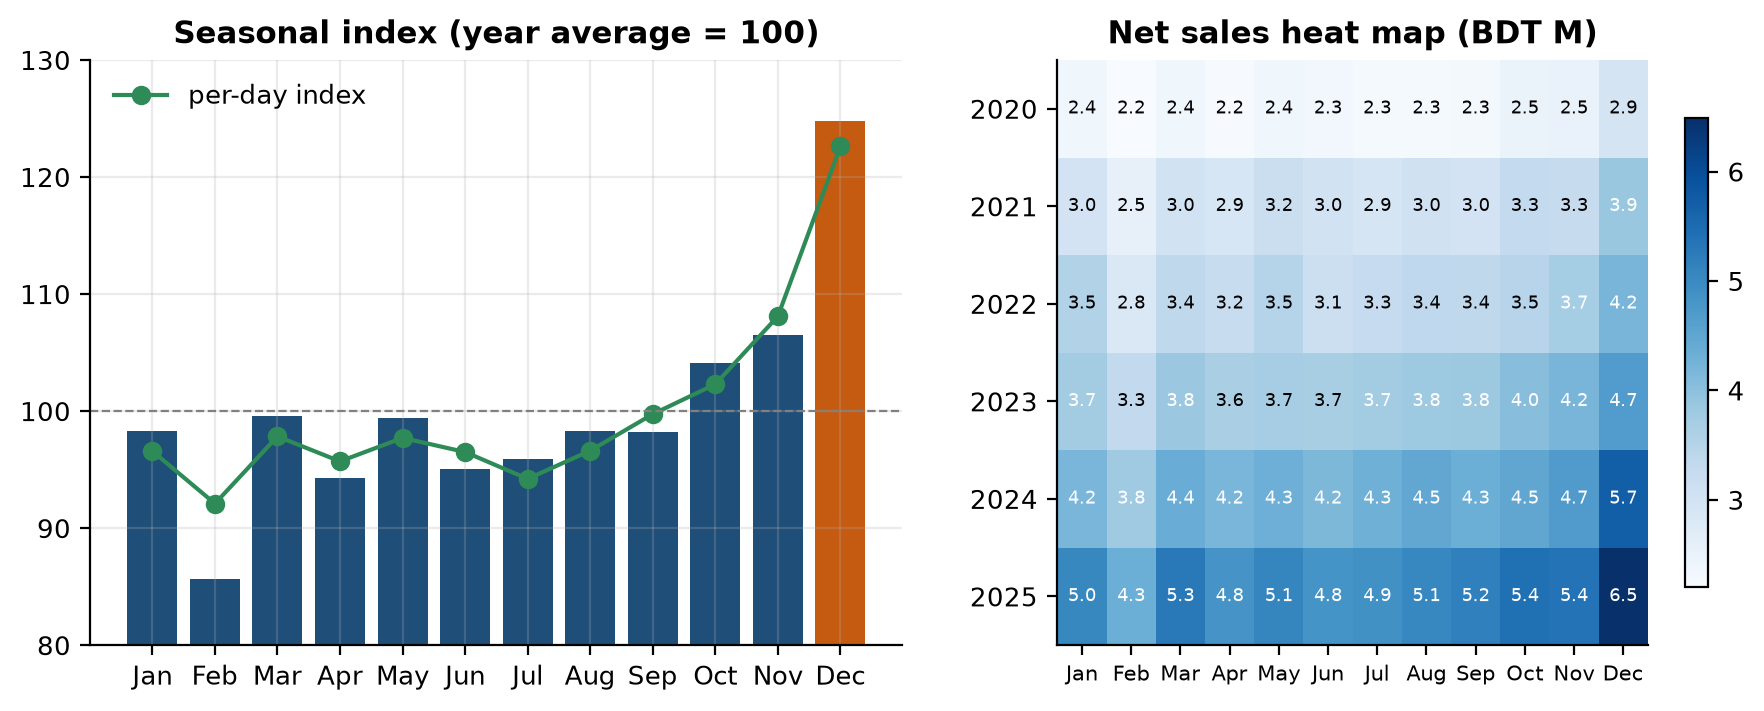
\includegraphics[width=\linewidth]{eda_seasonality}
\caption{Seasonal index by month (left) and year $\times$ month heat map of net sales (right)}\label{fig:seasonality}
\end{figure}

\section{Products and categories}
\Cref{tab:category} and \cref{fig:pareto} show the category structure. \TopCategory is the largest category
(\TopCategoryShare\% of sales), followed by Pound Cake and Swiss Roll. Layer Cake has the highest growth rate
(\FastCategoryCAGR\% a year). This growth comes mainly from gift-box variants added to the range in 2021, a
reminder that category growth figures combine organic growth with range changes. The Pareto analysis divides
the \NProducts products into \NClassA A-class products, which earn 80\% of revenue, and \NClassB B-class and
\NClassC C-class products. The ten best-selling products alone deliver \TopTenShare\% of net sales
(\cref{tab:topproducts}).

\begin{table}[htbp]
\centering
\small
\caption{Revenue and growth by product category}
\label{tab:category}
\begin{adjustbox}{max width=\linewidth}
\begin{tabular}{lrrrr}
\toprule
\textbf{Category} & \textbf{Net sales (BDT M)} & \textbf{Share \%} & \textbf{Products} & \textbf{CAGR 2020-25 \%} \\
\midrule
Muffin & 71.47 & 22.4 & 9 & +32.3 \\
Pound Cake & 61.76 & 19.4 & 12 & +9.7 \\
Swiss Roll & 38.81 & 12.2 & 4 & +9.6 \\
Fruit Cake & 28.90 & 9.1 & 5 & +9.9 \\
Layer Cake & 28.47 & 8.9 & 4 & +67.7 \\
Dry Cake & 25.59 & 8.0 & 3 & +9.4 \\
Cookie & 21.72 & 6.8 & 3 & +11.0 \\
Plain Cake & 16.57 & 5.2 & 6 & +10.4 \\
Velvet Cake & 11.75 & 3.7 & 1 & +10.3 \\
Classic Brownie & 6.27 & 2.0 & 1 & +10.8 \\
Premium & 4.02 & 1.3 & 1 & -- \\
Breakfast & 1.75 & 0.6 & 1 & -- \\
Bread & 1.28 & 0.4 & 2 & -- \\
\bottomrule
\end{tabular}
\end{adjustbox}
\par\smallskip\parbox{0.92\linewidth}{\footnotesize\emph{Note:} CAGR is computed between the first and last complete years. Categories launched after 2020 show growth from their launch year base.}
\end{table}
\begin{table}[htbp]
\centering
\small
\caption{Top ten products by net sales (Pareto/ABC analysis)}
\label{tab:topproducts}
\begin{adjustbox}{max width=\linewidth}
\begin{tabular}{lrrr}
\toprule
\textbf{Product} & \textbf{Net sales (BDT M)} & \textbf{Cumulative share \%} & \textbf{Class} \\
\midrule
MUF007 Cappuccino Muffin Gift Pack & 15.41 & 4.8 & A \\
MUF006 Vanilla Muffin Gift Box & 12.48 & 8.8 & A \\
LAY004 Vanilla Layer Cake Gift Box & 12.44 & 12.7 & A \\
LAY002 Chocolate Layer Cake Gift Box & 12.29 & 16.5 & A \\
MUF003 Chocolate Muffin Gift Box & 12.25 & 20.4 & A \\
MUF009 Chocochips Muffin & 11.99 & 24.1 & A \\
MUF008 Raisin Muffin & 11.80 & 27.8 & A \\
VEL001 Chocolate Velvet Cake & 11.75 & 31.5 & A \\
SWR002 Chocolate Swiss Roll & 11.68 & 35.2 & A \\
SWR004 Strawberry Swiss Roll & 10.44 & 38.5 & A \\
\bottomrule
\end{tabular}
\end{adjustbox}
\end{table}

\begin{figure}[htbp]\centering
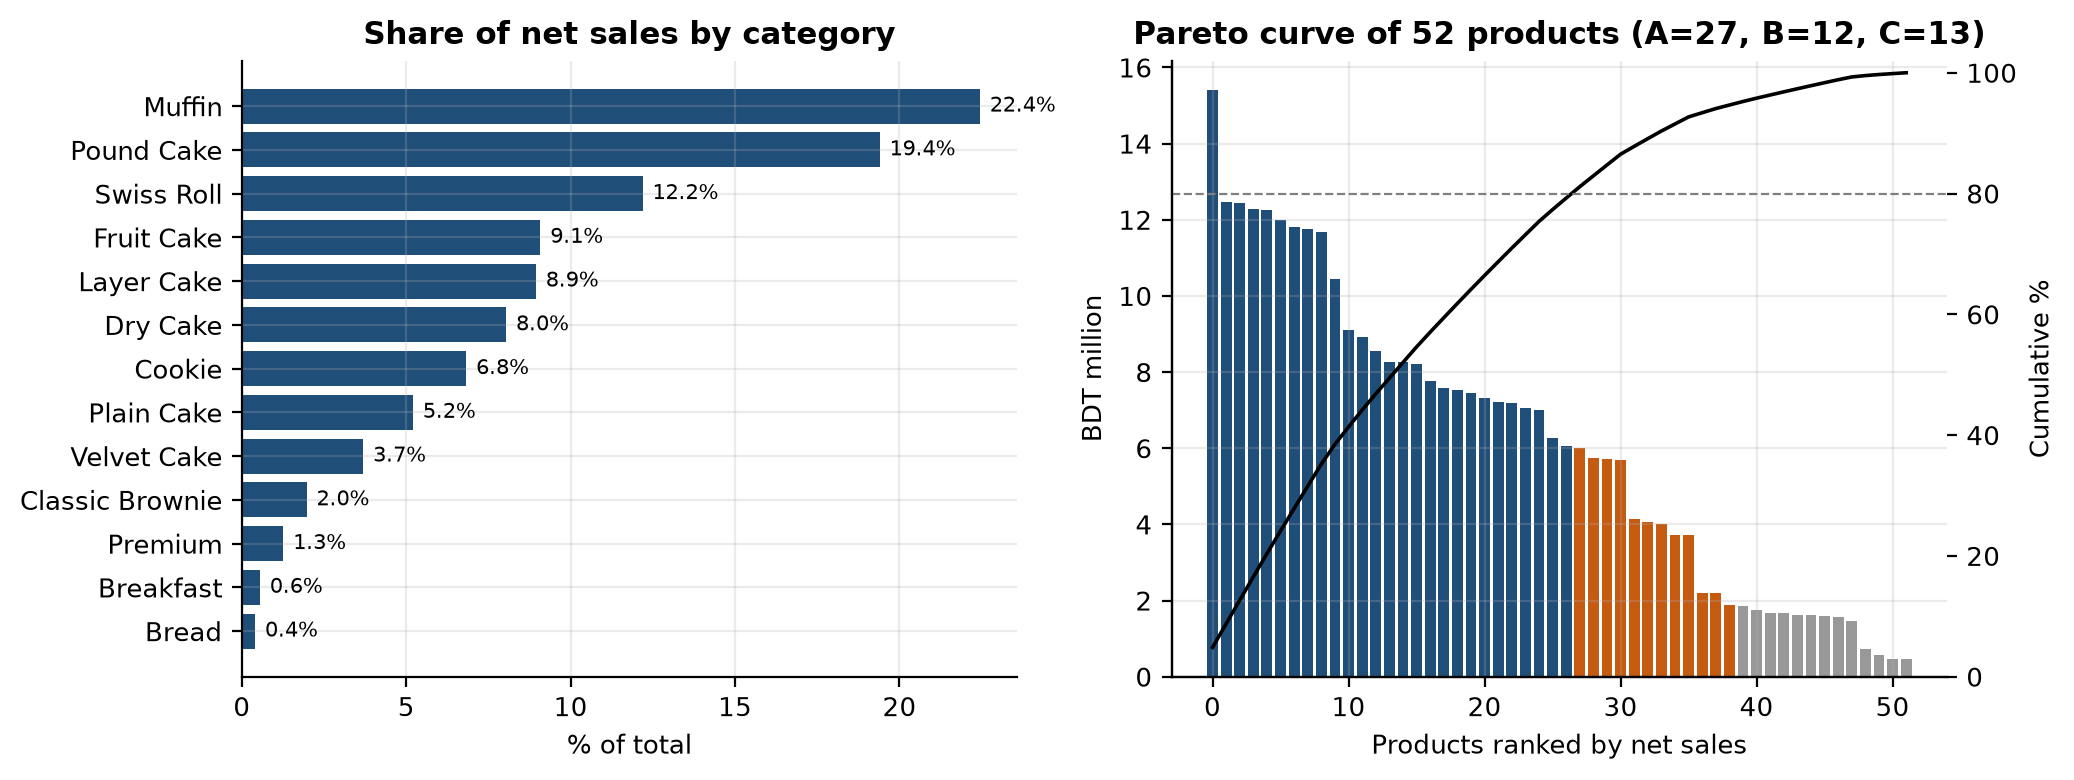
\includegraphics[width=\linewidth]{eda_category_pareto}
\caption{Share of net sales by category (left) and Pareto curve of products (right)}\label{fig:pareto}
\end{figure}

\section{Regions, channels and customers}
Sales are geographically concentrated. Dhaka generates \DhakaShare\% of net sales, and Dhaka and Chattogram
together \DhakaCtgShare\% (\cref{tab:segments}). General Trade is the main channel (\GTShare\%), followed by
Modern Trade (\MTShare\%), Distributors (\DistShare\%) and E-commerce (\EcomShare\%). The channels differ
sharply in order size. A distributor order averages \DistQty units, an E-commerce order \EcomQty, General Trade
\GTQty and Modern Trade \MTQty (\cref{fig:regionchannel}). Customer type, on the other hand, makes no difference
to order size (Kruskal--Wallis $p=\PCustType$), and average order values are almost identical across customer
types. Order size is therefore governed by the \emph{route to market}, not by who the customer is.

\begin{table}[htbp]
\centering
\footnotesize
\caption{Performance by region, channel and customer type}
\label{tab:segments}
\begin{adjustbox}{max width=\linewidth}
\begin{tabular}{llrrrrr}
\toprule
\textbf{Dimension} & \textbf{Level} & \textbf{Net sales (BDT M)} & \textbf{Share \%} & \textbf{Orders} & \textbf{AOV (BDT)} & \textbf{Units/order} \\
\midrule
Region & Dhaka & 139.76 & 43.9 & 169,661 & 823.8 & 7.85 \\
Region & Chattogram & 45.89 & 14.4 & 70,440 & 651.4 & 6.33 \\
Region & Gazipur & 25.74 & 8.1 & 39,853 & 645.9 & 6.34 \\
Region & Narayanganj & 21.23 & 6.7 & 35,195 & 603.1 & 5.93 \\
Region & Cumilla & 15.71 & 4.9 & 29,911 & 525.2 & 5.19 \\
Region & Sylhet & 15.27 & 4.8 & 29,901 & 510.6 & 4.92 \\
Region & Rangpur & 12.23 & 3.8 & 30,012 & 407.6 & 4.16 \\
Region & Rajshahi & 12.03 & 3.8 & 25,152 & 478.2 & 4.79 \\
Region & Khulna & 11.73 & 3.7 & 25,094 & 467.3 & 4.71 \\
Region & Mymensingh & 10.76 & 3.4 & 24,849 & 432.9 & 4.34 \\
Region & Barishal & 8.04 & 2.5 & 19,932 & 403.2 & 3.96 \\
Channel & General Trade & 145.21 & 45.6 & 260,431 & 557.6 & 5.32 \\
Channel & Modern Trade & 81.55 & 25.6 & 124,619 & 654.4 & 6.28 \\
Channel & Distributor & 72.90 & 22.9 & 64,861 & 1,123.9 & 11.43 \\
Channel & E-commerce & 18.72 & 5.9 & 50,089 & 373.7 & 3.66 \\
Customer type & Retailer & 143.28 & 45.0 & 224,582 & 638.0 & 6.19 \\
Customer type & Super Shop & 63.31 & 19.9 & 100,073 & 632.7 & 6.16 \\
Customer type & Distributor & 47.91 & 15.0 & 75,413 & 635.3 & 6.19 \\
Customer type & Online Customer & 31.95 & 10.0 & 49,759 & 642.0 & 6.17 \\
Customer type & Corporate & 31.93 & 10.0 & 50,173 & 636.4 & 6.21 \\
\bottomrule
\end{tabular}
\end{adjustbox}
\end{table}

\begin{figure}[htbp]\centering
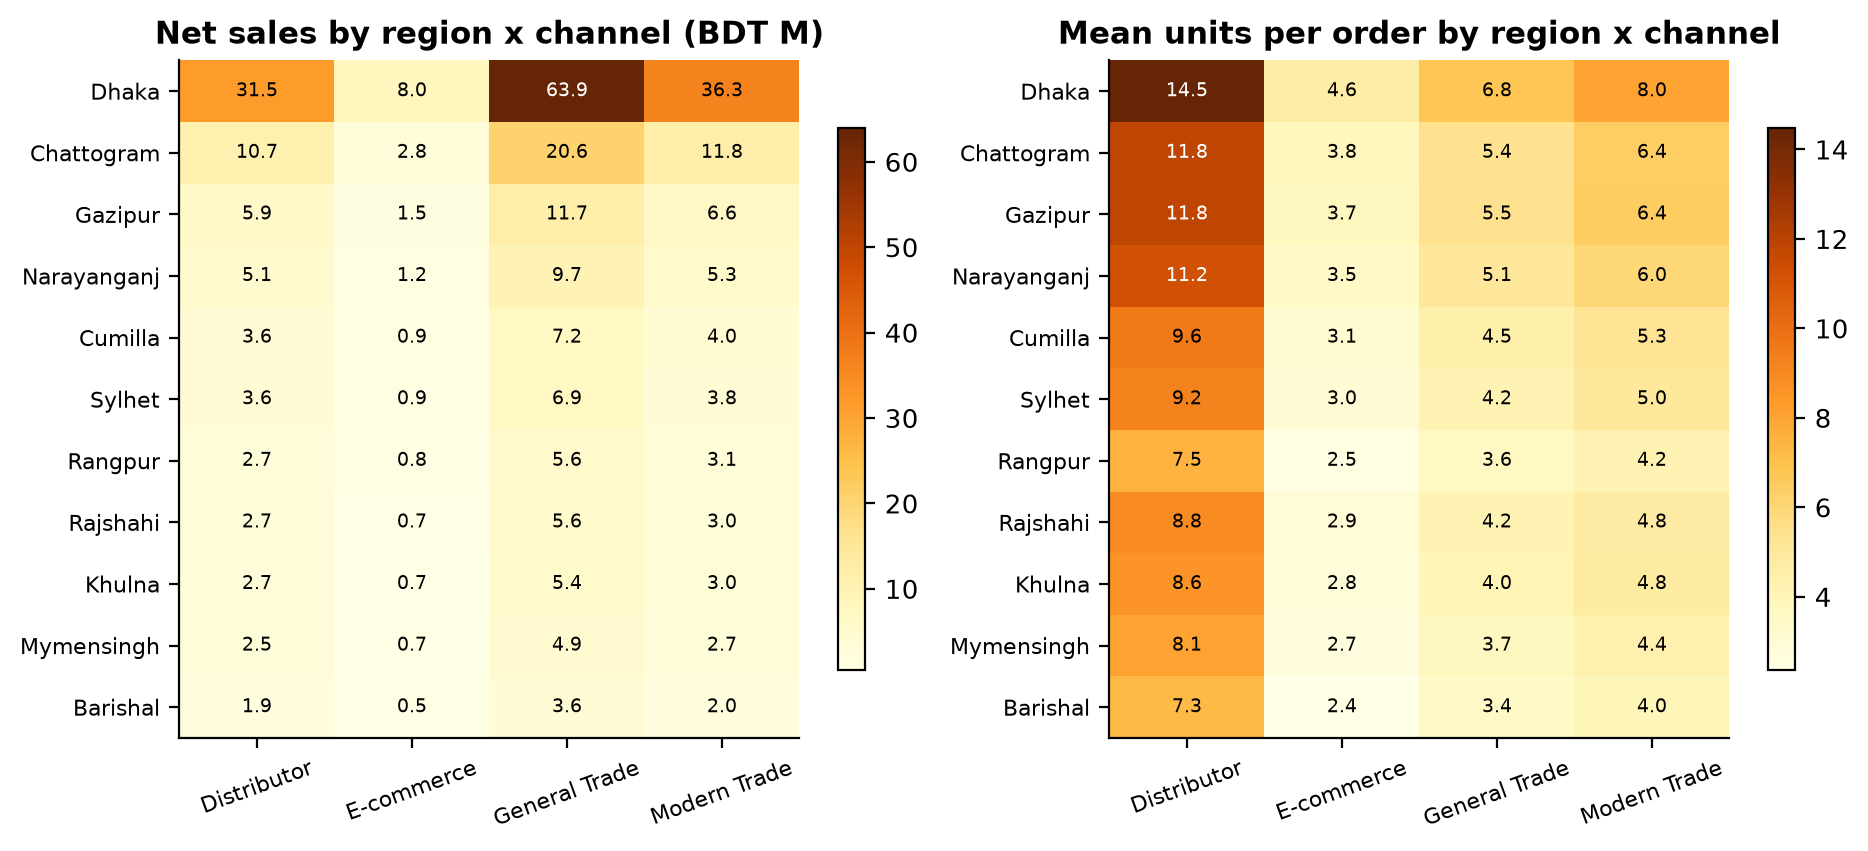
\includegraphics[width=\linewidth]{eda_region_channel}
\caption{Net sales (left) and mean units per order (right) by region and channel}\label{fig:regionchannel}
\end{figure}

\section{Distributions and relationships}
Order quantity and order value are strongly right-skewed, with skewness of \QtySkew and \ValueSkew
respectively (\cref{fig:distributions}). Most orders are small, and a long tail of bulk orders exists. These
shapes justify the use of medians, rank-based tests and log transformations throughout the analysis. The
Spearman correlation matrix (\cref{fig:correlation}) shows that order value is driven by both quantity
($\rho=\CorrSalesQty$) and price ($\rho=\CorrSalesPrice$). Quantity and price, however, are practically
unrelated ($\rho=\CorrQtyPrice$): customers do not buy fewer packs of the more expensive products.

\begin{figure}[htbp]\centering
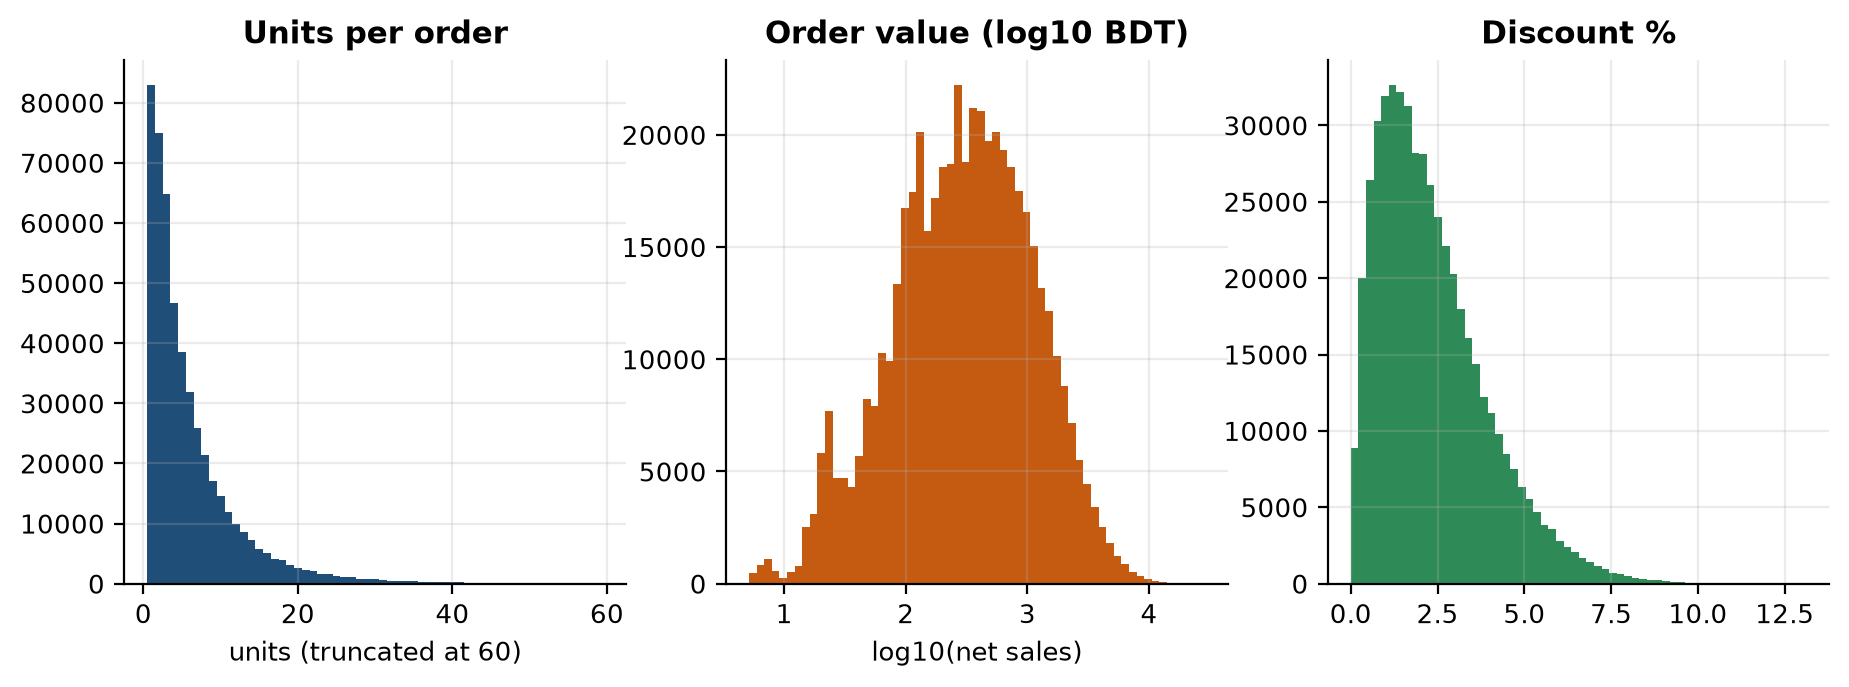
\includegraphics[width=\linewidth]{eda_distributions}
\caption{Distributions of units per order, order value (log scale) and discount}\label{fig:distributions}
\end{figure}

\begin{figure}[htbp]\centering
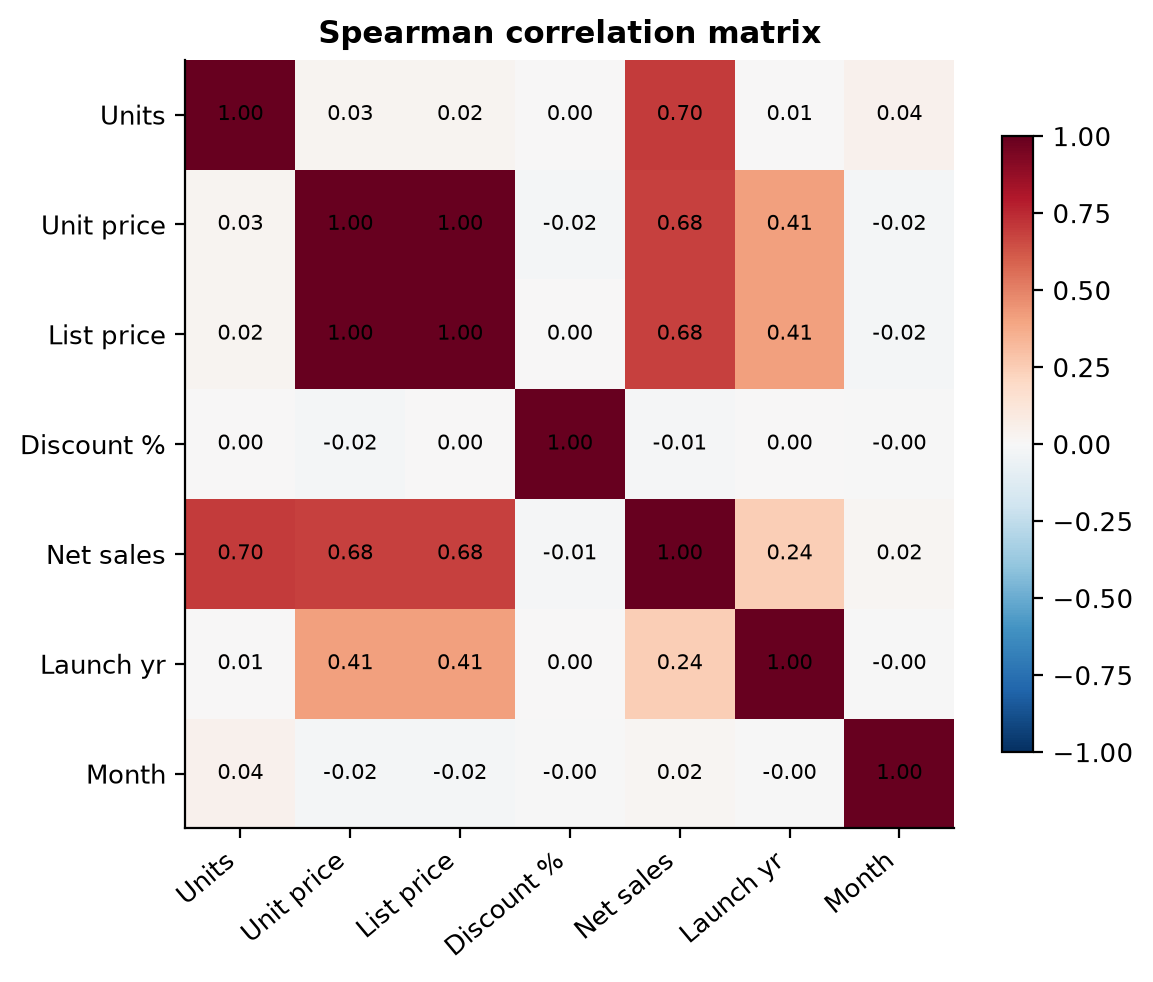
\includegraphics[width=.62\linewidth]{eda_correlation}
\caption{Spearman correlation matrix of the main numeric variables}\label{fig:correlation}
\end{figure}

\section{Hypothesis tests}
\Cref{tab:tests} formalises the main exploratory findings. With half a million observations, every difference
except two is statistically significant, so effect sizes are essential for interpretation. Channel explains the
most variation in order size ($\varepsilon^2=\EpsChannel$), followed by region ($\varepsilon^2=\EpsRegion$).
The association between channel and large orders is moderate (Cram\'er's $V=\CramerV$). Discount depth and
order size are \emph{uncorrelated} ($\rho=\RhoDisc$, $p=\PDisc$). The discounts given do not appear to
stimulate larger purchases. This is a potentially valuable finding, because discounts cost the company
\BDT\DiscountCost million over the period.

\begin{table}[htbp]
\centering
\small
\caption{Statistical tests of the main exploratory hypotheses}
\label{tab:tests}
\begin{adjustbox}{max width=\linewidth}
\begin{tabular}{llrrr}
\toprule
\textbf{Hypothesis (H0: no difference)} & \textbf{Test} & \textbf{Statistic} & \textbf{p-value} & \textbf{Effect size} \\
\midrule
Units/order by channel & Kruskal-Wallis & 43,269.88 & <0.001 & 0.0865 \\
Units/order by region & Kruskal-Wallis & 27,261.36 & <0.001 & 0.0545 \\
Units/order by customer type & Kruskal-Wallis & 2.62 & 0.623 & -0.0000 \\
Daily sales by month (detrended) & Kruskal-Wallis & 510.92 & <0.001 & 0.2293 \\
Discount \% vs units/order & Spearman rho & 0.00 & 0.479 & 0.0000 \\
Large order vs channel & Chi-square & 31,777.06 & <0.001 & 0.2521 \\
\bottomrule
\end{tabular}
\end{adjustbox}
\par\smallskip\parbox{0.92\linewidth}{\footnotesize\emph{Note:} Effect sizes: $\varepsilon^2$ for Kruskal--Wallis, $\rho^2$ for Spearman and Cram\'er's $V$ for chi-square. With $n=500{,}000$ almost any difference is `significant', so the effect size decides practical importance.}
\end{table}

\section{Summary of exploratory findings}
\begin{enumerate}
  \item Revenue growth is strong (\CAGRSales\% a year) but mostly price- and mix-driven; volume grows at \CAGRUnits\%.
  \item Demand is price-inelastic in the observed range, and discounts show no measurable effect on order size.
  \item Seasonality is pronounced, with a \PeakMonth peak and a \TroughMonth trough; weekdays do not matter.
  \item Revenue is concentrated: Dhaka provides \DhakaShare\% of sales and ten products provide \TopTenShare\%.
  \item Order size depends on channel and region, not on customer type.
\end{enumerate}
These findings informed the modelling choices in the next chapter. Seasonality and history features are used
for forecasting, channel and region for classification, and price, growth and seasonality for segmentation.
